\documentclass[journal]{IEEEtran}
\usepackage{blindtext}
\usepackage{graphicx}
\usepackage{cite}
\usepackage{multirow}
\usepackage{booktabs}
\usepackage{siunitx}
\usepackage[T1]{fontenc}
\usepackage[pdftex,breaklinks,pdfauthor={MSD Team P17101},pdfcreator={Philip Linden},pdftitle={P17101 Arcjet Thruster}]{hyperref}
\usepackage{nomencl}
\makenomenclature{}

% cite.sty was written by Donald Arseneau
% V1.6 and later of IEEEtran pre-defines the format of the cite.sty package
% \cite{} output to follow that of IEEE. Loading the cite package will
% result in citation numbers being automatically sorted and properly
% "compressed/ranged". e.g., [1], [9], [2], [7], [5], [6] without using
% cite.sty will become [1], [2], [5]--[7], [9] using cite.sty. cite.sty's
% \cite will automatically add leading space, if needed. Use cite.sty's
% noadjust option (cite.sty V3.8 and later) if you want to turn this off.
% cite.sty is already installed on most LaTeX systems. Be sure and use
% version 4.0 (2003-05-27) and later if using hyperref.sty. cite.sty does
% not currently provide for hyperlinked citations.
% The latest version can be obtained at:
% http://www.ctan.org/tex-archive/macros/latex/contrib/cite/
% The documentation is contained in the cite.sty file itself.

% http://edge.rit.edu/edge/P17101/public/Home

\title{P17101: Design and Characterization of a 1kW Arcjet Thruster Tabletop Technology Demonstrator}
\author{
  Philip~Linden$^{*}$\thanks{$^{*}$MEng Student, Department of Mechanical Engineering},
  James~Gandek$^{\dagger}$\thanks{$^{\dagger}$BS Student, Department of Mechanical Engineering},
  Dylan~Bruce$^{\dagger}$,
  Matt~Giuffre$^{\dagger}$,
  Anthony~Higgins$^{\ddagger}$\thanks{$^{\ddagger}$BS Student, Department of Electrical Engineering},
  David~Yin$^{\ddagger\S}$\thanks{$^{\S}$Only contributed to MSD I}
}
  % page header for pages other than cover page
  \markboth{P17101 Arcjet Thruster}%
  {Linden \MakeLowercase{\textit{et al.}}: Multidisciplinary Senior Design, RIT}

\begin{document}
\maketitle
% correct bad hyphenation here
\hyphenation{explor-ation explor-atory}

\begin{abstract}
A tabletop prototype of an arcjet electrothermal propulsion system was developed to supplement ongoing exploratory spacecraft development conducted by RIT Space Exploration (SPEX). The arcjet thruster demonstrates the degree of practicality in implementing electrothermal propulsion systems. The arcjet assembly generates an electrical arc across the thruster nozzle's throat, ionizing argon propellant in order to achieve a greater specific impulse compared to cold gas propulsion.
\end{abstract}

\label{sec:nomenclature}
% List all symbols and subscripts used for any math equations.
% This will add the units
%----------------------------------------------
\newcommand{\nomunit}[1]{%
\renewcommand{\nomentryend}{\hspace*{\fill}#1}}
%----------------------------------------------
% gas dynamics
\nomenclature{$A$}{Cross-sectional area of nozzle
  \nomunit{\,\si{\meter\squared}}}
\nomenclature{$p$}{Gas pressure
  \nomunit{\,\si{\kilo\pascal}}}
\nomenclature{$v$}{Gas flow velocity
  \nomunit{\,\si{\meter\per\second}}}
\nomenclature{$\dot{m}$}{Gas mass flow rate
  \nomunit{\,\si{\kilo\gram\per\second}}}
\nomenclature{$\alpha$}{Diverging nozzle half-angle
  \nomunit{\,\si{\deg}}}
% rocket equations
\nomenclature{$F$}{Thrust
  \nomunit{\,\si{\newton}}}
\nomenclature{$I_{sp}$}{Specific impulse
  \nomunit{\,\si{\second}}}
\nomenclature{$g_0$}{Standard acceleration due to gravity
  \nomunit{\,\SI{9.81}{\meter\per\second\squared}}}
\printnomenclature{}

\section{Introduction}
\label{sec:intro}
\IEEEPARstart{R}{IT} Space Exploration (SPEX) provided a hypothetical use-case to serve as the foundation for this exploration into satellite propulsion.
SPEX's hypothetical mission objective is to design a communicaitons satellite that is capable of maintaining a polar geostationary orbit for 10 years.

In practice, satellites in Earth orbit for long-duration missions in excess of 5--25 years encounter perturbations to their trajectories over time from residual atmospheric and orbital particles, or from variations in Earth's gravity field.
These spacecraft perform short station-keeping maneuvers periodically to compensate for drift and orbital decay.

An electrothermal rocket engine is method of propulsion by which an inert gas stored at ambient temperature (cold gas) is released from a pressurized vessel or driven by a pump and heated electrically before being expelled out of a nozzle.
Two proven methods of electrothermal propulsion are \emph{resistojets}, which use conventional heat exchangers to heat the propellant, and \emph{arcjets}, which pass the propellant through an electrical arc to heat the gas.

Electrothermal propulsion is advantageous over conventional chemical or cold-gas rockets for use by long-life satellites since the engines may be small in size, have no moving parts, and are more efficient at the expense of thrust.
While resistojets and arcjets require more elecrical power than chemical rockets, for example, the electrical energy may be recovered over time by photovoltaic panels, for example, whereas propellant fuel is a finite resource for these spacecraft.

A tabletop prototype thruster was designed and tested to explore the feasibility of this type of system with less strict requirements compared to the limitations of building a flight-worthy system.
A tabletop version does not require integration with a spacecraft, and mass and spatial limitations are relaxed.

\section{Design Theory}
\label{sec:method}
% Describe why an arcjet was selected over a resistojet.
In low power (\SI{1}{\kilo\watt}) applications, an arcjet offers up to 200\% gains in efficiency over a resistojet thruster~\cite{sutton2010rocket}.
\autoref{fig:power-vs-isp} identifies the typical use cases and performance characteristics of arcjets compared to various other types of electrothermal thrusters.
Arcjets achieve a greater specific impulse compared to resistojets but produce less thrust.
Thus a maneuver would take a longer amount of time using an arcjet but would consume less propellant overall for the same maneuver as compared to a resistojet.
\begin{figure}[htp]
  \centering
  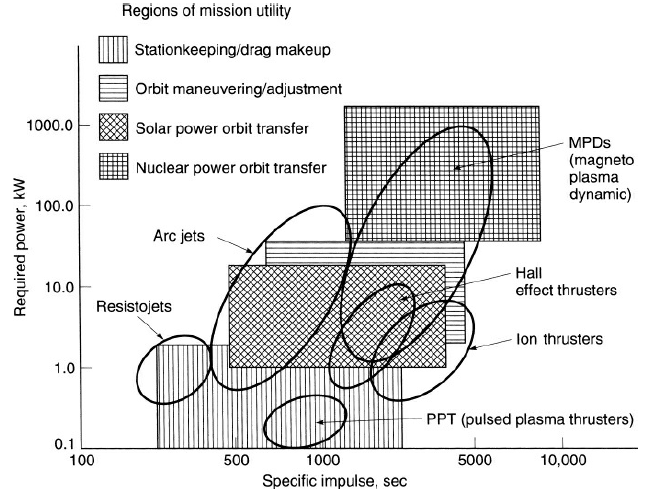
\includegraphics[width=\linewidth]{figs/power-vs-isp_sutton}
  \caption[Types of electrothermal propulsion]{There are various types of electrothermal propulsion with respect to typical performance and mission utility.
  In the \SI{1}{\kilo\watt} range, arcjets typically have a higher specific impulse than resistojets. (Sutton~2010)
\label{fig:power-vs-isp}}
\end{figure}

% Justify propellant selection (and explain paschen curve?)
The ideal propellant for arcjet engines is one which can be stored easily, has a low atomic mass, and favorable thermodynamic conditions during heating and expansion.
NASA identifies Hydrogen (H$_{2}$), Ammonia (NH$_{3}$), and Hydrazine (N$_{2}$H$_{3}$) as ideal propellants for arcjets~\cite{nasa1992considerations}.
Unfortunately, these gases are toxic or difficult to handle on a university campus.
Nitrogen (N$_{2}$) is an easy-to-handle alternative that has relatively favorable ionization and thermodynamic characteristics, and has been used in similar low-power arcjet demonstrations~\cite{olin2012report,olin2012sim}.
% High level gas dynamics analysis
\begin{figure}[htp]
  \centering
  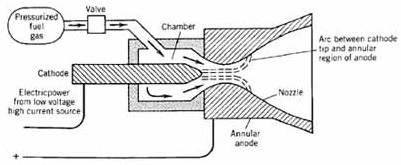
\includegraphics[width=\linewidth]{figs/cross-section_nasa}
  \caption[Arcjet cross-section]{A cross sectional view of a typical arcjet shows the expected flowpath of propellant and the expected region of the electric current arc. The propellant is ionized and heated by the arc then expanded through the nozzle. (NASA~GRC~1992)
\label{fig:x-section-nasa}
}
\end{figure}

Gas enters the chamber and is ionized and heated by a high-current arc that extends from the cathode to the throat of the anodic nozzle to form a plasma.
In the ideal case, the plasma reaches sonic speed in the throat and is supersonically accelerated as it expands through the nozzle.

Thrust is a function of the momentum of the flow exiting the nozzle.
\begin{equation}
\label{eq:thrust}
  F=\dot{m}v_e + (p_e-p_b)A_e
\end{equation}
 Where $F$ is thrust, $\dot{m}$ is mass flow rate of propellant, $v$ is flow velocity, $A$ is nozzle cross sectional area of the nozzle, and subscript $e$ denotes parameters at the nozzle exit while $p_b$ denotes atmospheric backpressure.
 In space, $p_b$ is negligible and the thruster is design around such condition.

 A thruster's efficiency is described in terms of specific impulse, $I_{sp}$, which may be used to compare performance with other space propulsion methods.
 \begin{equation}
 \label{eq:isp}
   I_{sp}=\frac{F}{\dot{m} g_0}
 \end{equation}
% some calculations?
In the ideal condition using gaseous N$_2$ as propellant, a conical nozzle with $\alpha=50$ is capable of \SI{0}{\newton} of thrust without a sustained arc.
At sea-level, \SI{0}{\newton} of thrust is expected.

<<<<<<< HEAD


\section{System Overview}
% outline the main system architecture.

\subsection{Engine}
\begin{table}[hbp]
  \caption{Theoretical thrust and Isp values with respect to space and sea-level operation, total pressure $p_0= $\SI{20}{psi}.
\label{tab:theoretical-performance}
}
  \begin{tabular}{lrrrrr}
    \toprule
    & & \multicolumn{2}{c}{Without arc} & \multicolumn{2}{c}{With arc} \\
    & $p_b$ (\si{\kilo\pascal}) & Thrust (\si{\newton}) & $I_{sp}$ (\si{\second}) & Thrust (\si{\newton}) & $I_{sp}$ (\si{\second}) \\
    \midrule
    Vacuum & $0$ & $0$ & $0$ & $0$ & $0$ \\
    Sea-level & $101.3$ & $0$ & $0$ & $0$ & $0$  \\
    \bottomrule
  \end{tabular}
\end{table}

% how much energy transferred from arc to plasma?

\section{System Overview}
% outline the main system architecture.
\subsection{Thruster}
% Describe the main components of the thruster and how they interact. Be sure to include material selection justifications. Show some basic analysis and predictions for performance with justification.
Propellant flows into an aluminum body and is spun into a vortex about the tip of the cathode, where it passes through an electric arc before being accelerated through a conical nozzle.
The flow swirler is a high-temperature thermal insulator.
The high-temp insulator and cathode are mounted concentrically into a low-temperature PTFE thermal and electrical insulator, which is fixed to the thruster test stand.
The nozzle is electrically insulated from the aluminum body by a non-cunductive spacer.
\begin{figure}[htp]
  \centering
  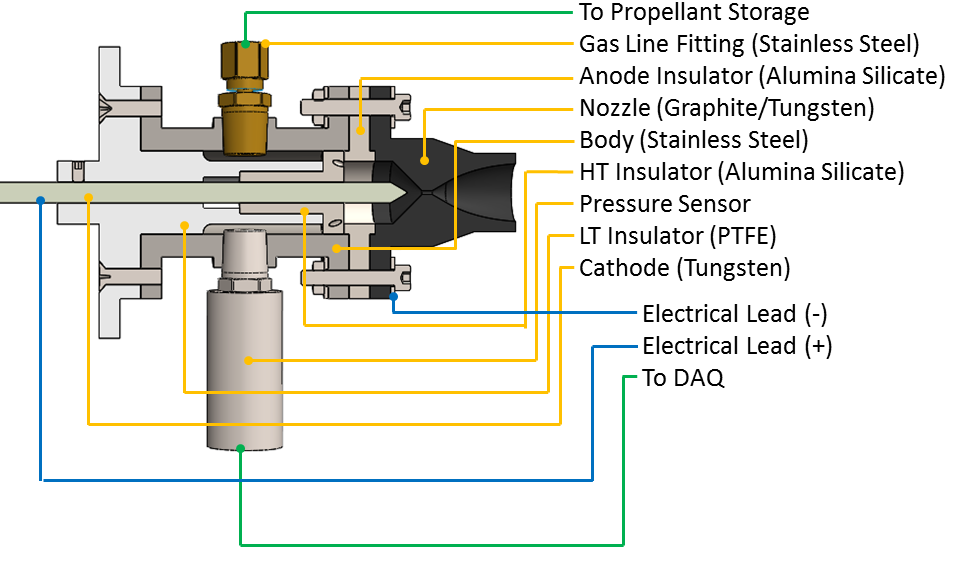
\includegraphics[width=\linewidth]{figs/cutaway_annotated.png}
  \caption[P17101 Arcjet Annotated Cutaway]{Components that are charged or exposed to extreme heat are electrically and thermally insulated.
\label{fig:annotated-cutaway}
}
\end{figure}

\subsection{Power Conditioning Unit}
% Describe the inputs and desired outputs of the unit. Explain the theoretical justification behind the HV/HC approach. Describe the approach in theoretical terms and list practical limitations.
The electrical arc used to add energy to the gas is generated and sustained by the Power Conditioning Unit (PCU).
The PCU consists of high-voltage (HV) and high-current (HC) modes.
The HV side of the circuit initiates the arc, then the PCU switches to the HC ``side'' of the circuit to sustain a high-current arc.
This architecture is similar to a plasma torch and has been demonstrated in similar tabletop systems~\cite{park2015thesis}.

% explain HV side here
\SI{120}{\volt} AC power is supplied to the HV side of the circuit, then the voltage is increased by a series of voltage doublers. A tungsten rod serves as the cathode of the HV circuit, and the graphite nozzle of the thruster acts as the anode.
% explain HC side here
When the arc jumps between the cathode and anode across the flowpath, it closes the HC portion of the circuit. This current induces a redd switch to open, turning off the HV side of the PCU.\@


\subsection{Data Acquisition \& Control}
% Explain the DAQ hookup and justification for the DAQ, and limitations to that choice. Show and describe the VI\@.

% explain HV side here
\SI{120}{\volt} AC power is supplied to the HV side of the circuit and converted to DC by dimmable light switch.
The supplied voltage is increased to \SI{45}{\kilo\volt} by an automotive ignition coil.
A tungsten rod serves as the cathode of the HV circuit, and the graphite nozzle of the thruster acts as the anode.
High voltage across the gap between anode and cathode generates an arc, effectively shorting the HV circuit.

\begin{figure}[htp]
  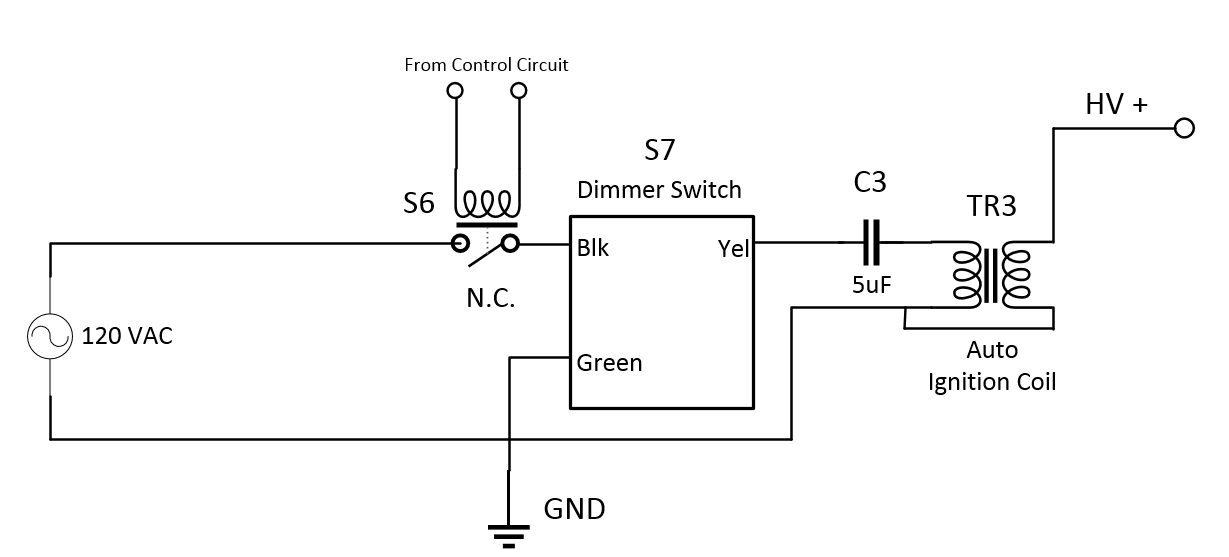
\includegraphics[width=\linewidth]{figs/hv-schematic.png}
  \caption{Wall AC power is converted to DC high voltage in order to initiate an arc.
\label{fig:hv-circuit}
}
\end{figure}

% explain HC side here
When the arc jumps between the cathode and anode across the flowpath, current induces a reed switch to open, opening the HV side of the PCU and completing the HC side of the circuit.
\emph{Anthony, please explain how the high current components are structured to condition supply power to high current.}
\SI{0}{\ampere} flows through the arc between anode and cathode.

\begin{figure}[htp]
  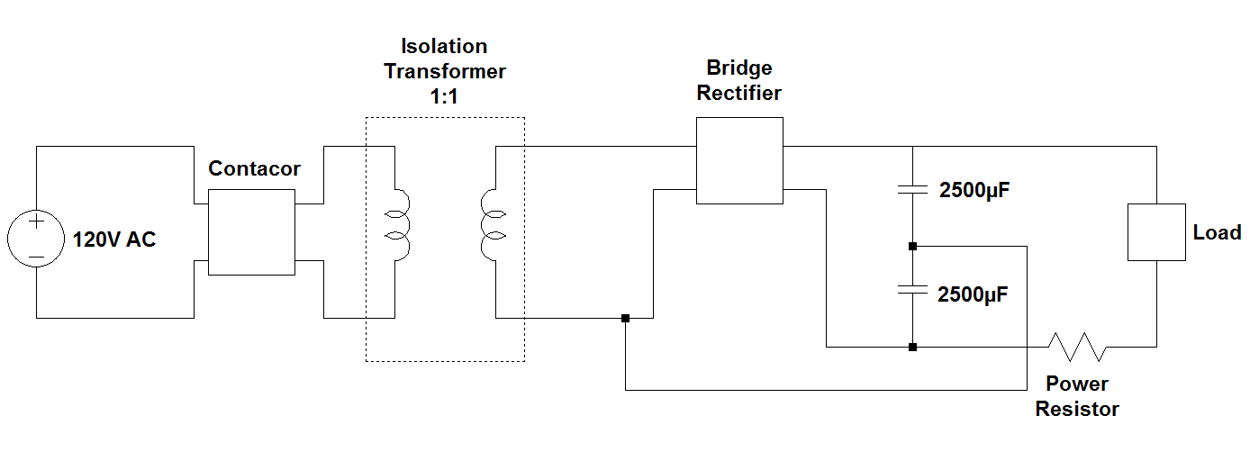
\includegraphics[width=\linewidth]{figs/hc-schematic.png}
  \caption{Anthony, please explain the high current circuit here.
\label{fig:hc-circuit}
}
\end{figure}

During a burn, the PCU draws $900$--$1100$\si{\watt} from the wall outlet.

\subsection{Test Stand}
% Explain the physical apparatus that measures the system's outputs. Describe the interactions between the thruster and the test stand. Justify instrumentation selection.
The thruster is mounted to a lever arm with its exhaust facing upward.
The opposite arm of the lever is connected to a $0$--$0$\si{\newton} load cell.
The weight of the thruster offsets the ``zero'' load condition such that it is sufficiently far from the sensor's floor.
When a burn is underway, thrust force is measured as a change from the equilibrium condition.
The [Brand Name] load cell was selected for its high resolution, as this was more cost effective than purchasing a low-force load cell.

Propellant is supplied by a gaseous nitrogen dewar at \SI{0}{psi}.
The GN$_2$ is regulated to \SI{0}{psi} before reaching a normally-closed solenoid valve.
GN$_2$ is flowed through the system for several seconds before PCU ignition to ensure only nitrogen is present in the thruster, and after PCU shutdown to cool hot hruster components.

\subsection{Data Acquisition \& Control}
% Explain the DAQ hookup and justification for the DAQ, and limitations to that choice. Show and describe the VI.
Operation of the PCU and propellant solenoid is nominally controlled by a Texas Instruments MyDAQ and LabVIEW Virtual Interface (VI).
The test engineer starts and stops a test with the VI from a computer connected to the test stand. The timing of solenoid and PCU events may be programmed or toggled manually.

The MyDAQ device also collects data from all sensors used in the test stand.
Thruster performance is quantified by measuring thrust force generated during a burn.
Pressure inside the main body is monitored to judge the health of the system during operation and saved as a secondary performance metric.

\subsection{Test Stand}
% Explain the physical apparatus that measures the system's outputs. Describe the interactions between the thruster and the test stand. Justify instrumentation selection.

\subsection{Safety Measures}
% Describe risk management in more detail. Consider ommitting this section~\cite{linden}.
In the event of a computer malfunction, an emergency shutoff button is wired into the circuit between the outlet and the PCU and the solenoid is normally closed and non-latching.
When a test is conducted, the test stand is placed in a well-ventilated Formula SAE engine test cell, and the control computer is located outside the testing room.
The VI monitors sensor data in real-time and shuts down operation when sensor parameters reach unsafe limits.

% Because of some charring observed in the plywood base during circuit operation, an informal test was performed on the power resistors under operational conditions to gain an estimate on the temperature changes over time.
% The graphs below show the average temperature increase is 7.4F per second. The charring temperature of wood is 250-300F, and a 10s burn would require a temperature buffer of 80-90F.
% In order to protect the wood enclosure a temperature cutoff was added to the power line that opens at 250F.

\section{Test Procedure}
% Describe the basic test plan in broad terms and how we approached testing. Describe the setup within the engine test cell and how the user interacts with the system.

\section{Results}
% Show results and how they compare to our predictions. Describe any failures and the problem solving process that occurred.

\section{Conclusions \& Recommendations}
% Evaluate the success of the project and make recommendations for improving it.

\section*{Acknowledgments}
The team thanks Mr.~Vincent Burolla for his unwavering support; the Mechanical Engineering Department, the Multidisciplinary Senior Design Department, and the Kate Gleason College of Engineering for their resources and workspaces; RIT Space Exploration and Boeing for sponsoring this project.

\bibliographystyle{IEEEtran}
\bibliography{p17101}

\end{document}
